% $Id: template.tex 11 2007-04-03 22:25:53Z jpeltier $

\documentclass{vgtc}                          % final (conference style)
\let\ifpdf\relax
%\documentclass[review]{vgtc}                 % review
%\documentclass[widereview]{vgtc}             % wide-spaced review
%\documentclass[preprint]{vgtc}               % preprint
%\documentclass[electronic]{vgtc}             % electronic version

%% Uncomment one of the lines above depending on where your paper is
%% in the conference process. ``review'' and ``widereview'' are for review
%% submission, ``preprint'' is for pre-publication, and the final version
%% doesn't use a specific qualifier. Further, ``electronic'' includes
%% hyperreferences for more convenient online viewing.

%% Please use one of the ``review'' options in combination with the
%% assigned online id (see below) ONLY if your paper uses a double blind
%% review process. Some conferences, like IEEE Vis and InfoVis, have NOT
%% in the past.

%% Figures should be in CMYK or Grey scale format, otherwise, colour 
%% shifting may occur during the printing process.

%% These three lines bring in essential packages: ``mathptmx'' for Type 1 
%% typefaces, ``graphicx'' for inclusion of EPS figures. and ``times''
%% for proper handling of the times font family.

\usepackage{mathptmx}
\usepackage[pdftex]{graphicx}
\usepackage{times}
\usepackage{epstopdf}

%% We encourage the use of mathptmx for consistent usage of times font
%% throughout the proceedings. However, if you encounter conflicts
%% with other math-related packages, you may want to disable it.

%% If you are submitting a paper to a conference for review with a double
%% blind reviewing process, please replace the value ``0'' below with your
%% OnlineID. Otherwise, you may safely leave it at ``0''.
\onlineid{0}

%% declare the category of your paper, only shown in review mode
\vgtccategory{Research}

%% allow for this line if you want the electronic option to work properly
\vgtcinsertpkg

%% In preprint mode you may define your own headline.
%\preprinttext{To appear in an IEEE VGTC sponsored conference.}

%% Paper title.

\title{ADetector: An interactive visual analytic tool for time-series climate anomaly data detection}

%% This is how authors are specified in the conference style

%% Author and Affiliation (single author).
%%\author{Roy G. Biv\thanks{e-mail: roy.g.biv@aol.com}}
%%\affiliation{\scriptsize Allied Widgets Research}

%% Author and Affiliation (multiple authors with single affiliations).
%%\author{Roy G. Biv\thanks{e-mail: roy.g.biv@aol.com} %
%%\and Ed Grimley\thanks{e-mail:ed.grimley@aol.com} %
%%\and Martha Stewart\thanks{e-mail:martha.stewart@marthastewart.com}}
%%\affiliation{\scriptsize Martha Stewart Enterprises \\ Microsoft Research}

%% Author and Affiliation (multiple authors with multiple affiliations)
\author{Tsung Tai Yeh\thanks{e-mail: yeh14@purdue.edu}\\ %
     \parbox{1.4in} \scriptsize Electrical Computer Engineering Department \\ Purdue University %
\and Shuying Feng\thanks{e-mail:feng98@purdue.edu}\\ %
     \parbox{1.4in}\scriptsize Electrical Computer Engineering Department \\ Purdue University %
%\and Martha Stewart\thanks{e-mail:martha.stewart@marthastewart.com}\\ %
%     \parbox{1.4in}{\scriptsize \centering Martha Stewart Enterprises \\ Microsoft Research}
}

%% A teaser figure can be included as follows, but is not recommended since
%% the space is now taken up by a full width abstract.
%\teaser{
%  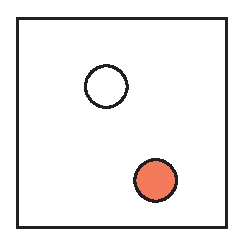
\includegraphics[width=1.5in]{sample.eps}
%  \caption{Lookit! Lookit!}
%}

%% Abstract section.
\abstract{Data quality plays an important role on the data analysis results. However, finding and fixing anomaly data is time-consuming in big data. There should be a systematic approach to narrow down the data checking regions. In addition to the expected abnormal data, such as missing data, and extreme data, the time-series data also includes some unpredictable and latent erroneous data. The patterns of unpredictable data are difficult to predict and recognize. We present ADetector, a visual analytic tool for anomalies identification in complex and large time-series datasets. This tool applies the nonlinear regression model to fast locate potential anomalies in big tim-series data, introduces a novel data representation of comic map grid for anomalies analysis to identify anomalies. ADetector exploits visual analytics interface and iterative anomaly detection pipeline to pick out possible latent abnormal data. From the time-series weather data anomaly analysis, the correlation of approximate regression model is highly positive, and ADetector is able to complete anomaly analysis tasks over 10 years time-series data in less than one minute.   
} % end of abstract

%% ACM Computing Classification System (CCS). 
%% See <http://www.acm.org/class/1998/> for details.
%% The ``\CCScat'' command takes four arguments.

%\CCScatlist{ 
%  \CCScat{Anomaly detection}%
%{Time-series data};
%  \CCScat{Time-series data}
%}
\keywords{time-series data, anomaly detection, visual analytics}

%% Copyright space is enabled by default as required by guidelines.
%% It is disabled by the 'review' option or via the following command:
% \nocopyrightspace

%%%%%%%%%%%%%%%%%%%%%%%%%%%%%%%%%%%%%%%%%%%%%%%%%%%%%%%%%%%%%%%%
%%%%%%%%%%%%%%%%%%%%%% START OF THE PAPER %%%%%%%%%%%%%%%%%%%%%%
%%%%%%%%%%%%%%%%%%%%%%%%%%%%%%%%%%%%%%%%%%%%%%%%%%%%%%%%%%%%%%%%%

\begin{document}

%% The ``\maketitle'' command must be the first command after the
%% ``\begin{document}'' command. It prepares and prints the title block.

%% the only exception to this rule is the \firstsection command
\firstsection{Introduction}

\maketitle

%% \section{Introduction} 

	The precision of measurement plays an important role in scientific experiments and engineering systems, since the mistakes of the measurement often cause disastrous consequences. For instance, the confusion about the value of the fuel led to the failure of NASA Mars Climate Orbiter in 1999, and the A Boeing 767 aircraft ran out of gasoline in mid-flight\cite{ifan2012}. However, errors embedded in the scientific measurements are inevitable due to the experimental uncertainties or malfunction of apparatus. For example,  many inputs are either human-generated or unstructured data (e.g. user logs, tweets, comments on social networks), or assessment data from sensors (thermometers, scales, DNA sequencers) including measurement errors. 

	Error analysis aims to measure the quality of the scientific experiments and engineering systems, find out abnormal data hidden in a set of measurements, and get rid of these unexpected errors. However, it is not easy to figure out uncertain errors hidden in the big amount of data, and analyzing the complete set of data could be computationally expensive. The results from a thorough analysis of this big data may not be worth the cost for completeness. In addition, we are not able to know what the exact value is in the measurement. However, in fact, we can make sure the correct value exists in a specified likelihood\cite{ifan2012}. Thus, an approximate clue from big data is supposed to be enough for us to obtain perfect answers to pinpoint errors similar to results from a thorough analysis.
	
	The great numbers of uncertainties in the measurement increase the challenge of error diagnosis due to the limited erroneous data knowledge base. In general, the taxonomy of anomaly in the scientific experiments includes random errors, systematic errors, and mistakes. The impact of random errors on the precision of the measurement in which indicates the experimental results are close to the average one in the repeated measurements. For instance, the malfunctioned instrument often leads to the fundamental random noises, and cause the bad degree of precision. Furthermore, the systematic error means the measurement quantity is inaccurate, which is away from the accepted or predicted values. For example, the interference arises from environment often distract the measurement results from the expected one. The last one is the mistakes, which is often caused by some unpredictable conditions such as incorrect manual records, and is difficult to detect. These hatred errors could be solved by integrating visual representation, data analysis, and human interaction.

	
	The least-square fitting methods, regression model and signal processing filters are often used to measure the relationship between two or more phenomena. The residual value among variables is usually being a baseline to estimate outliers included in a set of measurement. Furthermore, the previous research always pursue a best-fit model to predict or estimate the trends or patterns of data. However, the computational costs and convergence speeds of these curve fitting methods are getting to be a concern in big data analysis. In fact, the amount of noises or errors is usually less than the correct ones in various applications. In other words, the noise is not the principle characteristics of the measurement. In addition, we never obtain the exact measurement and the erroneous patterns are often shift away from the expected value. Thus, an approximate solution is enough to diagnose the experimental data. In this paper, we present an approximate nonlinear regression -- matching pursuit, which integrate Fourier Transform and approximate least square method for anomaly inference.

	Visual analytics is used to reduce the size of data analysis, to audit the data, and to detect anomaly interactively. Even if statistical inference methods are helpful for the recognition of abnormal data, however, some kinds of spurious data which are hard to be recognized by numerical model. For instance, the small glitch, or a series stark unchanged measurement. The visualisation enables human-beings to extract additional characteristics via data comparison efficiently. Moreover, the statistical evidence and view highlights allow people to determining a specified region of data that is susceptible to errors to check and avoid the thorough analysis. We present an anomaly visual analytics pipeline, and a data comparison graphical interface -- comic map to take insight into the complex measurement data.
	
	In addition to the data reduction supports, visual exploration tool also includes the visual comparison functionality. Stack zooming \cite{javed2010stack} exploits the stack hierarchy to serve as a tangible graphical history to proceed the visual comparison. In constast with stack zooming, the comic map visual comparison we used in our anomaly detection tool unrestrains the direction or hierarchy of visual comparison. Comic map provides more freedom for users to cluster cells with the similar attributes, and merge multiple variables in one cells to compare data, and understand the characteristics of time-series data easily. In general, exploring, querying, and comparing are steps to figure out the patterns of anomaly hidden in time-series data.
		
In sum, this paper includes the following contribution. 

1. The approximate nonlinear fitting curve model: This model combines signal processing approach, and leverages fitting curve to predict abnormal data hidden in time-series climate data.  
 
2. Visual analytics pipeline for anomaly detection: Showing the possible abnormal data in line graph comic map cells, and exploits various interactions such as zoom in/out, swapping, and merging to allow human-being recognize abnormal data patterns.

3. Visual anomaly exploration, and timeline showcase: Time is a nice clue to understand the time-seris data. Hence, we support the a visual timeline navigation to explore the abnormal data.    

\section{Background}

\subsection{Anomaly data classification}

The category of time-series anomaly is opt to the objective, and monitoring procedure of data collection. The time-series data we are focus on is weather data sets, which are collected by MesoWest weather data service settled by University of Utah. MesoWest weather data service collects numerous weather data such as temperature, humidity, and wind pressure etc.. at thousands of locations around the United States, and provides weather history records over 10 years at each measurement locations. According to the observation of the weather data from MesoWest service, we sum up time-series anomaly in weather data as follows.

{\bf a. Missing data} results from unexpected status of climate sensors, and causes the value of collecting data becomes null. The problem of the missing data is to interrupt the numerical calculation in data analysis, and to induce the wrong analysis results. Thus, the missing data is often removed before the start of data analysis via data clean tool. However, the missing data occurrence frequency, and time record can be the inferrence of abnormal data, and evaluation of the status of measure instruments. 

{\bf b. Extreme data} is the outlier \cite{rousseeuw2005robust}in a set of time-series data. The extreme data can be undermined by the robust data analysis. Although the outlier is often looked as an anomaly in signal processing or image processing, since many environmental factors influence the change of the weather data patterns, the extreme data is not always an error in climate data sets. The spurious extreme data impacts on the accuracy of results of analysis. However, to visualize the extreme data is able to help for finding additional characteristics in the weather data sets. In addition, time-series visual comparison is also helpful for anomaly judgement.
 
{\bf c. Latent abnormal data} indicates some unpredictable data and even the regression model is hard to discern this type of error. For instance, the small glitch or a set of unchanged measurement occurred in a continuous time interval. The latent abnormal data influence the precision of the measurement, and cause the incorrect trend estimation. The visualization is an efficient approach to understand the fluctuation of time-series data, and figure out more characteristic about latent abnormal data.

\subsection{Time-series visual exploration}

Considerable visual analytics research which is related to the time-series visual visualization, and exploration, and the relevant surveys include \cite{silva2000visualization}. The basic line graph \cite{tufte1983visual}is widely in temporal visualization. However, in recent year, in order to delve into the time-series, different visual representation techniques have been worked out\cite{bremm2011interactive}, \cite{mclachlan2008liverac}, \cite{javed2010stack}, \cite{sip2012}, \cite{Liao2010}, \cite{Liao2011}. These graphical representation methods improves the efficiency and effectiveness for time-series data analysis. Furthermore, the massive time-series visual analytics has also became a consideration in ATLAS \cite{chan2008maintaining} system.
 
	Query and exploration also plays a key role in time-series visual analytics. LifeLine\cite{plaisant1996lifelines} is an eary visual system for personal history record exploration. TimeSearcher\cite{hochheiser2004dynamic} is an interactive time-series query tool, and uses the time-box to explore the data sets. PatternFinder \cite{fails2006visual} includes an visual interface to query the medical records. LiveRAC \cite{mclachlan2008liverac} designed an interactive visual interface to explore the data collected from computer systems. Data quality assessment is also getting to become an important topics in visual analytics research. Profiler\cite{Kandel2012}, and RainMon\cite{shafer2012rainmon} integrated statistical analysis and visual representation to find out abnormal hidden in database and computer systems. 
	
	The above projects concentrate mainly on the interactive visual explorations, and visual representation for time-series data. However, beyond the high-level visualization tasks, temporal visual exploration also requires additional attention to the pipeline of the data analytics for special properties. In particular, additional important time-series visual analytics tasks include (a) multi-variable relationship (b) dynamic time-series hierarchies (c) large-scale support\cite{javed2010stack}. Few of the above visualization tools support all these requirement, except Stack Zooming\cite{javed2010stack}, and Live RAC\cite{mclachlan2008liverac}. 
	
\subsection{Support multi-focus comparision}

	The anomaly is the one that does not follow well defined normal behavior\cite{Chandola2009}. Anomaly is often unveiled via comparison with expected values or baseline model. Thus, we argue the temporal analysis is supposed to support the concept of multi-focus comparison. Multi-focus comparison framework is consist of the comparison tasks for the multiple focus, context, and distance awareness \cite{javed2010stack}, \cite{elmqvist2008melange}. This approach is supported by Stack Zooming\cite{javed2010stack}, which leverages one-dimensional nature of the data to present hierarchies of visualization strips, and LiveRAC \cite{mclachlan2008liverac}. In this paper, we take advantage of different approach to multi-focus interaction compared to Stack Zooming and LiveRAC system. We leverage comic map which is composed of multiple small cells, and integrate with the types of anomaly and timestamps to present the relationship of anomaly and its occurrence time. 
	
\subsection{Support collaboration and data reduction}

	Kittur et al\cite{kittur2008crowdsourcing} claims crowdsourcing is a successful approach, which depends on the intelligence of a group of human-beings to solve some hard problems. Furthermore, the distributed cognition\cite{liu2008distributed} has been showed the power to amplify sensemaking in the team-working analysis. The anomaly visual analytics tool is supposed to take the collaboration into consideration, since the mathematical model cannot understand all uncertainties embedded in time-series data. Thus, the participant in the team analysis can be a key role for anomaly exploration.
	 
	The scalability is getting to become a critical issue in big data visual analytics. It is hard to display all big data, because the overwhelming computational and memory overhead. The visual analysts can help to narrow down the size and range of data analysis based on the statistical view recommendation. In this paper, we work out a new visual analytics pipeline, which enable analysis participants join the iterative anomaly detection, and set up a possible abnormal time-series range to explore anomaly.


\section{ADetector}

ADetector is an anomaly visual exploration tool. Since the overwhelming anomaly detection costs in the massive data sets, ADetector combines an approximate statistical regression model, anomaly diagnostics, and visual analytics to narrow down the size of anomaly analysis, take insight into the complex structure of errors, and at last unveil abnormal data. Thus, ADetector is consist of data clean, reduction and comparison widgets to tackle on the time-series weather anomaly detection, and convey possible anomaly data to visual analysts to figure out the patterns of anomaly collaboratively.

\subsection{Anomaly diagnosis workflow}

In order to take insight into the patterns of abnormal data. ADetector takes advantage of an interactive visual anomaly detection pipeline to infer unpredictable anomaly. Thus ADetector is composed of five steps -- Data Table, Type inference, Anomaly region search, view recommendation, and interactive time-series navigation, and comparison.
 \begin{figure}[htb]
	\centering
  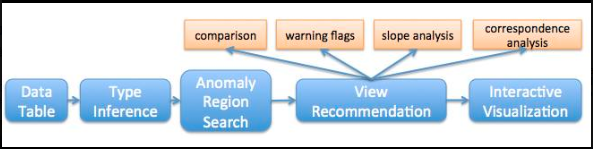
\includegraphics[width=0.49\textwidth]{workflow.png}
  \caption{The anomaly detection workflow of ADetector tool}
\end{figure}


Data table includes a series data manipulation options such as the selection of input and the type of weather data. Since ADetector tackles on missing, extreme, and latent anomaly, in the type inference step provides options to specify one of anomaly, then ADetector will use the specified analysis tool to analyze the selected one. Afterward, in the anomaly region search step, based on the selected anomaly, ADetector leverages statistical analysis to work out some statistical results that are related to the behavior of data to let users select a certain time interval (e.g. one year) to delve in to the micro-level. At last step, ADetector exploits regression model to carry out anomaly matching calculation, then show the possible anomaly region in multiple cells. The missing, extreme data statistics are showed in timeline widget, and users also can pick out data in one of time interval to view in cells in comic cells. Altogether, ADetector workflow is composed of selection, reduction, and comparison steps.

\subsection{The composition of ADetector}
\subsubsection{Data clean tool}

Data clean tool aims to find out all missing data in the data sets and show their timestamp. Users are able to figure out the occurrence frequency and time from this data clean tool. Furthermore, users also can remove the missing records from this data clean tool. Altogether, the data clean tool gives users an overview of the information about missing data, and allows users to remove them. 

\subsubsection{Abnormal region reduction tool}

The purpose of possible abnormal region reduction tool is to narrow down the data checking. This tool is composed of several histogram, and show the proportion of multiple statistical analysis results in each year. ADetector give three view recommendations including the number of missing data, the average of extreme data, and the residual between raw data, and fitting curve model to help users determinate which year is supposed to pay attention to. Afterward, users can delve into one specific year, and take a look at the monthly distribution. In the meantime, according to view recommendations. Users can choose one month to proceeds micro-analysis.

\subsubsection{Data comparison tool}

The data comparison tool consists of comic map, which includes multiple line graph cells. Importing the selected monthly data from susceptible abnormal region reduction tool, ADetector proceeds residual calculation toward selected data, and show a number of possible abnormal region in each comic map cells. In addition, this tool also supports cell switch and multiple line graph merge functionalities. From this tool, users are able to compare the fluctuation of each comic map cell. Furthermore, ADetector data comparison tool also includes stack zooming functionality. Users can select one certain time interval to zoom in and zoom out. 

% \begin{figure}[htb]
%\centering
%  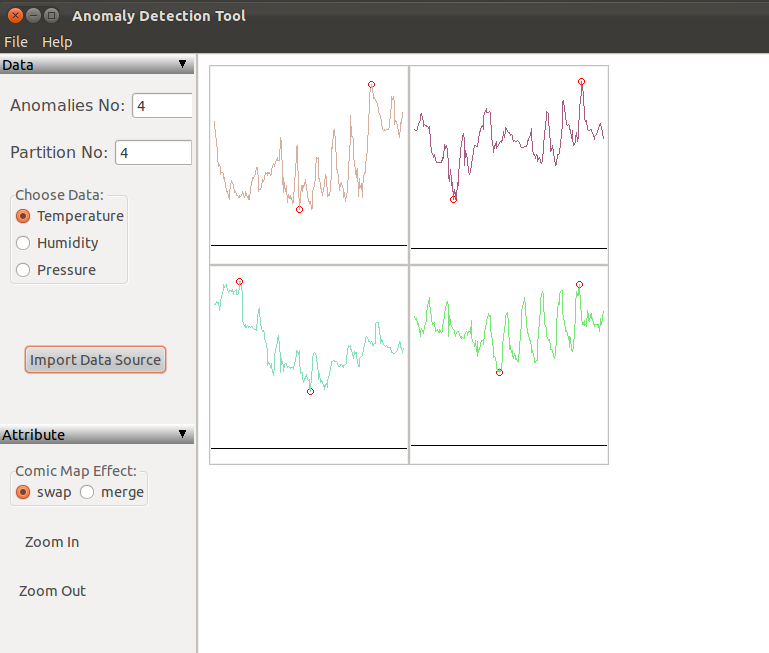
\includegraphics[width=0.49\textwidth]{comic.png}
%  \caption{Comic Map data comparison tool}
%\end{figure} 
\section{Comic Map Visual Representation}

After getting the potential anomalies from the computer, users can step in to analyze the potential anomaly in order to identify if it is actually an anomaly or to find out the reason for the anomaly. In time-series climate data, for example, some abnormal temperature may imply some useful climate phenomena in a specific time frame. In order to find out the pattern or trend behind these anomalies, it is useful to provide the users some method to compare the anomalies. Also an overview of the relationship of these anomalies with the whole datasets will help the users establish an overall understanding as well. Here we introduce a novel representation of anomalies – comic map. 

 \begin{figure}[htb]
	\centering
  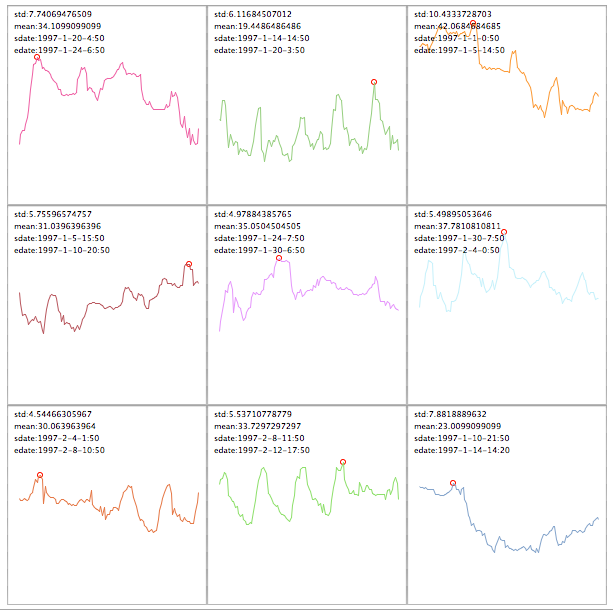
\includegraphics[width=0.45\textwidth]{comicMap9Cell.jpg}
  \caption{Comic Map}
\end{figure}

Comic map is composed of several grid cells. Each shows detail information of each anomaly (Figure 2). With this layout, user can swap and merge cells freely to compare the anomalies with simple drag-and-drop functionality. Moreover, An overview timeline representation of all anomalies is also established corresponding the comic map grid to give the user more knowledge of the anomaly based on the overall timeline (Figure 3)

 \begin{figure}[htb]
	\centering
  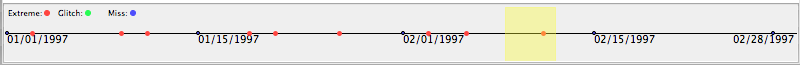
\includegraphics[width=0.45\textwidth]{timeline.png}
  \caption{Comic Map Timeline Overview}
\end{figure}

\subsection{Comic map cells}

The basic component of the comic map is every comic map cell. For time series data, a timeline-based representation is more intuitive for user to receive. And also in order to better understand the anomaly, the data surrounding this anomaly is needed for the user to get a picture of the trend of this anomaly, like for extreme anomaly, it appears much higher than other data around. So in each cell, anomaly data is shown along with some more data before and after it in a time sequence visualized as line graphs. In addition, the anomaly data is marked with a red circle as shown in Figure 4. 

 \begin{figure}[htb]
	\centering
  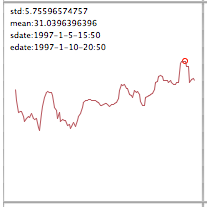
\includegraphics[width=0.20\textwidth]{onecell.jpg}
  \caption{Comic Map Cell}
\end{figure}

Other than the basic line graph of anomaly, some additional information is provided as plain text shown in the upper left corner of the cell, including standard deviation, mean value, start date of the data in this grid and end data of this grid cell. There is no axis along with timestamp labels is shown due to the space limit of the grid cell. Then the start date and end date is given to provide the user the information about the time. All these information are trying to help analyst get a better understanding of the dataset in the cell.
\subsection{Layout}
Cells of comic map are laid out as comic book grid (Figure 2). In this way, each cell has three (corner cell), five (edge cell) or eight neighbors around it. This kind of layout is more helpful for comparison. Since usually users prefer to set objects side by side to compare it. In our layout, each cell can be easily compared with their neighbors and the number of neighbors is bigger than the traditional horizontal or vertical layout. This is efficient since analyst can do more comparison in comic map layout with less cells moving around.

The comic map tries to maintain a layout more like a square, which is not only efficient of using the visual space, but also guarantees the aggregation of cells for comparison mentioned before. For example, if there are 4 anomalies in total, a 2x2 comic map will be shown, and if the anomalies number is 9, the comic map is a 3x3 grid. More specific, comic map will be chosen as the closest square based on anomalies number. For example, anomalies number between 10 and 16 results in a 4x4 grid.

Moreover, in order to reduce the work of swap, our backend model sorts all anomalies by putting anomalies with similar pattern besides each other. During analysis process, analyst can also rearrange cells for comparison by simply swapping cells. Our layout is very flexible, which provides the analyst a lot of freedom.

\subsection{Timeline overview}

For each cell, some information related to the specific anomaly can be obtained, but analyst still lacking information of this anomaly related to the whole dataset. So we introduce a timeline overview corresponding to the comic map grid (Figure 3). 
Since the dataset is a time-series climate data, time information should be an understandable choice for an overall representation. In the timeline overview, an axis of timestamp is used as the main visualization. Some timestamps are shown to give analyst an overview of time. On the time axis, anomalies are marked corresponding to their happening time. Specifically, different type of anomalies are marked using different colors. Through this overview visualization, analyst gains information of anomalies based on the whole dataset, like the frequency of anomaly in a specific timeframe, the occurrence of different type of anomalies, etc. 
The comic map cells are also tightly connected with this timeline overview. When a comic map cell is selected, the corresponding timeframe of data in the cell will be highlighted in the overview. More information can be obtained for analyst to analyze anomaly in the cell (Figure 5). 

 \begin{figure}[htb]
	\centering
  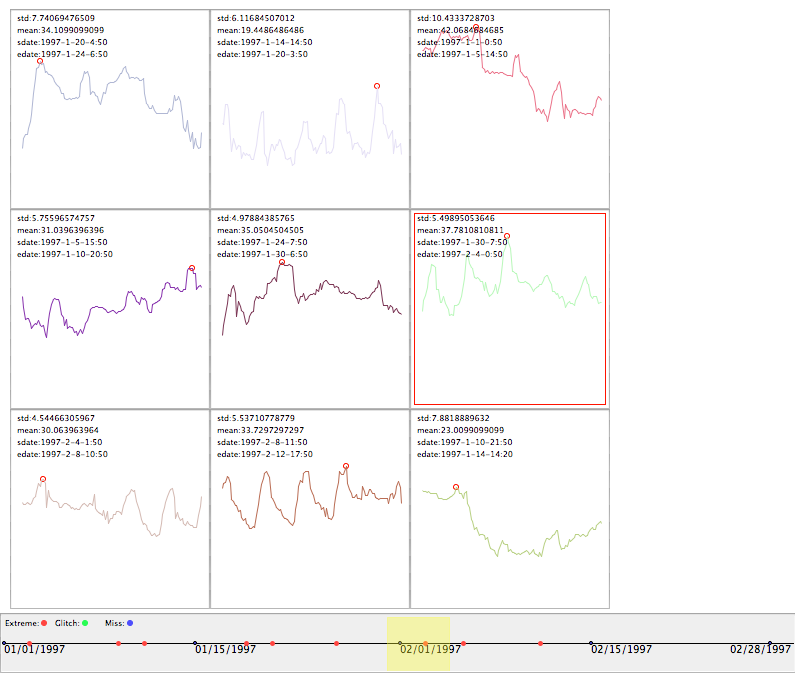
\includegraphics[width=0.45\textwidth]{timeline2.png}
  \caption{Timeline overview: select a cell, the corresponding time will be highlighted (light yellow)}
\end{figure}

\subsection{Comparison interaction}
As mentioned before, comparison plays an important role in anomaly analysis. Our comic map visual representation provides advanced interactions to support comparison, which gives the analyst more freedom of doing comparison and increases the efficiency of analyzing process.

\subsubsection{Swap}
The first interaction for comic map is swap. Analyst can swap any two cells by simply drag and drop. By using this interaction, analyst can put any cells beside to do a comparison.  Also, analyst can rearrange the comic map to put similar anomalies together (Figure 6).  

 \begin{figure}[htb]
	\centering
  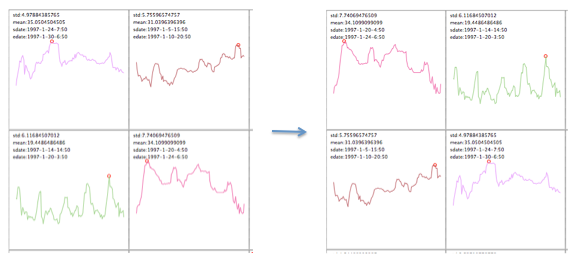
\includegraphics[width=0.45\textwidth]{swap.jpg}
  \caption{Comic Map Swap: upper-left cell swapped with lower-right cell, upper-right cell swapped with lower-left cell}
\end{figure}

\subsubsection{Merge}
The second interaction for comic map is merge. Comparison can be done by putting objects side by side, but can also be done shown two datasets in one view. The introduction of merge interaction enables the ability of doing comparison in one cell. 
In order to merge two cells into one cell, analyst can just pick up one cell and drag-and-drop it onto the cell that he wants to merge with. For example, if the analyst wants to merge first, second and third cell, he can drag-and-drop the first cell to the third cell, and then drag-and-drop the second cell to the third cell. A merged view is automatically generated in the third cell (Figure 7).

 \begin{figure}[htb]
	\centering
  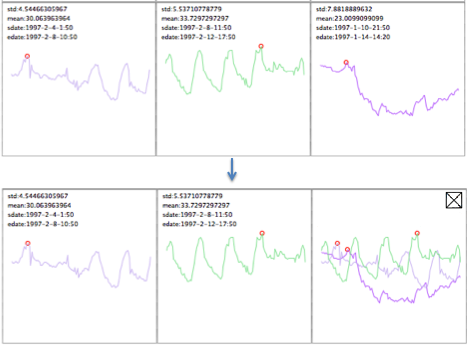
\includegraphics[width=0.45\textwidth]{merge.jpg}
  \caption{Comic Map Merge: first cell and second cell merged into third cell}
\end{figure}
 
The merged view is also revertible. There is a cross sign on the upper-right corner of the merged view. Simply by clicking the cross sign, the merged view will be reverted back to the original dataset view. For example in our former example, after clicking the cross sign, the third cell will show the original anomaly data in that cell (Figure 8).

 \begin{figure}[htb]
	\centering
  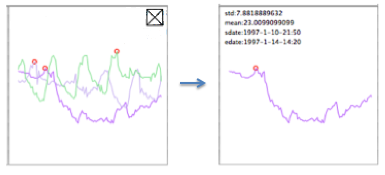
\includegraphics[width=0.45\textwidth]{merge2.jpg}
  \caption{Comic Map Merge: revert back to original data by clicking the cross sign}
\end{figure}

\subsubsection{Stack zooming}
The third interaction for comic map is stack zooming. Analyst often needs to see closer to the anomaly by zooming. The way of doing zooming in our comic map representation is stack zooming.

In order to zoom in a specific subset of data, analyst select the region (stack) he wants to zoom in (Figure 9). Then the cell will be automatically updated showing that portion of data. 
The same as merge interaction, stack zooming is also revertible by just clicking on the cross sign on the upper-right corner. Then, the original whole dataset of anomaly will be shown.

 \begin{figure}[htb]
	\centering
  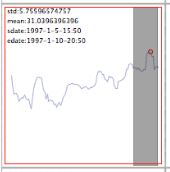
\includegraphics[width=0.20\textwidth]{zoom.jpg}
  \caption{Comic Map Merge: select a region (stack) to zoom}
\end{figure}

\section{Matching pursuit -- regressive anomaly detector}

Regression analysis is used to estimate the trends among variables with the change of the time. Regression analysis model is often used to predict or interrept observed data. Matching is one nonlinear regression model used in ADetector to figure out possible anomaly. The role of regression model is being a baseline to account for the data, and distinguish anomaly from normal one. Least-square fitting curve aims to work out a best-fit formula to describe the distribution or behavior of data. Linear regression model such as ordinary least squares, and weighted least square. However, these linear models sometimes are not applied in nonlinear time-series data, such as financial data, and weather data. In order to find out anomaly from massive data, the nonlinear regression model is supposed to meet scalable, low complexity, and feasible requirements.

\subsection{Approximate nonlinear regression model}

Fourier transform is a well-known tool in engineering and science. The amplitude in the frequency domain is able to represent the characteristic of the data in the time domain. Supposed that the noise is not the principle feature in the data, so the amplitude of noise is low. In addition, Fourier transform can be looked as a noise filter, since in the Fourier frequency domain, high amplitudes usually gather in the initial frequency. Thus, our objective is to leverage the top k big amplitude to reconstruct a fitting curve to estimate the anomaly. 

Matching pursuit is composed of the following five steps. The first step is to use Fourier transform to convert time-series input data to frequency domain. The second one is to obtain the frequency index of top k high amplitude to be the training data. Since the estimate data is consist of the scalar A, and the Fourier Transform equation, but A is unknown. Thus, in order to get the A scalar, the least square method is used to to get the scalar of A. After getting the number of A, the next step is to use scalar A1 to Ak to work out the number of k eigensolutions. At last, supperpositing these k eigen-solutions and carry out an approximate model that is closed to the original one.

\begin{figure}[htb]
\fbox{
	\centering
  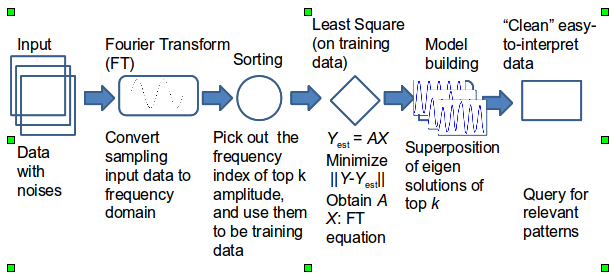
\includegraphics[width=0.45\textwidth]{fft.png}
	}
	\caption{The workflow of matching pursuit regression model}
\end{figure}

The advantages of matching pursuit regression model is it uses the number of frequency to build up the nonlinear fitting curve, and reduce the computational analysis costs. Furthermore, matching pursuit is non-parameter or unsupervised learning algorithm, there is no any training data requirement. At last, matching pursuit algorithm is also scalable, because it can be run in divide-and-conquer approach and in parallel way. Matching pursuit regression model provides us a rapid method to estimate the anomaly in massive time-series data. 

\subsection{Anomaly diagnostic logics}
	Only matching pursuit regression model is not enough to figure out the location of anomaly, since matching pursuit is like a ruler, there is supposed to be a method to figure out how to use this ruler to measure.
	
		(a) Systematic error: the systematic error is a bias that is shift away from the mean. According to the residual formula, we can calculate studentized residual between real data, and model one to figure out the outliers. ADetector use residual obtained from the matching procedure, and determine possible anomaly.
			
	\begin{equation}
	 res_i = \sigma^2 ( 1 -\frac{1}{n} \frac{((x_j - \overline(x)^2))}{\sum_i(x_j - \overline(x)^2))}
	\end{equation}		 
		(b) Latent anomaly data: Latent anomaly data is easy to unaware of because the characteristic of this anomaly is not revalent. In order to look for this anomaly, we calculate heteroskedasticity, and use cook's distance to understand the influential relation between real data and model, and visualize them in comic map cells. 

\section{Results}

We have conducted the eveluation of A-Dector on the time-series weather data collected from Meso weather service website. Meso time-series weather data service keeps over 17 years at different locations around the United States. We now want to validate the relationship between the degree of approximate and the quality of matching pursuit nonlinear regression model. In addition, we also want to figure out the analysis performance of this model, and the effectiveness of this model.

\subsection{The correlation validataion}

	In this validation, we want to see the performance of the anomaly detection in different size of data sets. 

Mean square error (MSE) is often used to account for the difference between two variables. In addition, Pearson correlation coefficient is used to measure the linear correlation between two variable. In this experiment, we input 3 year time-series weather data (the total number is 14600), and we change the number of k (the number of iteration) in the model construction, then measure the variations of MSE and Pearson correlation coefficient. 
\begin{figure}[htb]
\fbox{
	\centering
  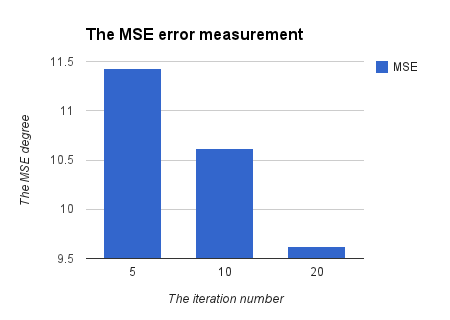
\includegraphics[width=0.23\textwidth]{chart_1.png}
  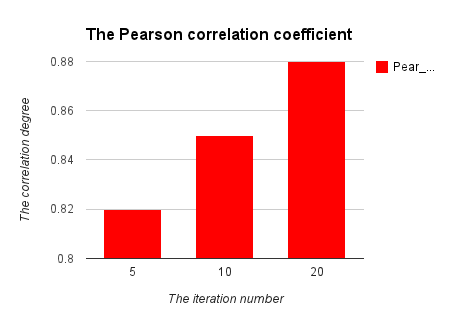
\includegraphics[width=0.23\textwidth]{chart_2.png}
	}
	\caption{The MSE and Pearson correlation coefficient}
\end{figure}

	At first, we can find the correlation in each experiemnt result reveal positive correlation, which means the model data is correlated to the real data. Furthermore, we also find the correlation coefficient is high when we only iterate the regresion algorithm 5 times. In other words, even the number of iteration is small, the degree of correlation is high positive. Second, we also conduct the MSE measurement, and we found the MSE decrease with the number of iteration, but the completion time increases with the growth of iteration.
	
\subsection{The performance validation}
In this validation, we want to see the performance of the anomaly detection in different size of data sets. We can see A-Detector can complete the anomaly data less than one minute. 

\begin{figure}[htb]
\begin{center}
\fbox{
	\centering
  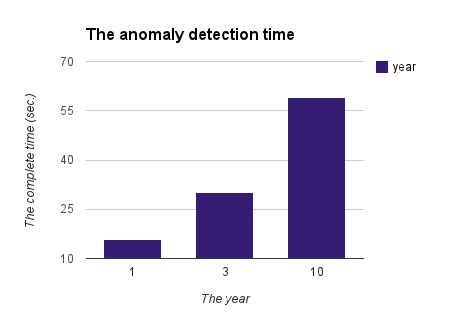
\includegraphics[width=0.30\textwidth]{chart_3.png}
	}
\end{center}
	\caption{The workflow of matching pursuit regression model}
\end{figure} 

\section{Future works}

In future work, we plan to support adaptive model tuning based on the feedback from users in the anomaly detection process. Currently in our tool, the anomaly detection model is totally processed in backend and users don’t have any control on it. Users can only compare the anomalies detected by the backend model, determinate whether it is really a anomaly by comparison and finally decide to delete it or not. So in order to give uses the ability to refine the backend model, we can let user add new parameters or change the value of parameters of the model (like correct data range, slope, etc) after finding out anomalies from visual graph.

      Moreover, for the data representation in the current version of our tool, we only support data aggregation in the overview window. For example, the overview of year shows first, if user clicks on a year data, detailed monthly data shows up. But in analyze workspace, an overview map only shows up for monthly view.  We may continue investigate a suitable aggregation representation in the analyze workspace map representation as well, which can give the user a better view of the whole structure for analyzing anomalies data as well.  
\section{Conclusion}

In this paper, we introduced a theoretical regression model, and a practical implementation of multi-focus comparison technique called comic map. The quality of data play a critical role in scientific and engineering systems, because errors often cause catastrophic consequence. However, in order to meet the requirement of a mountain of data, we should rethink the anomaly detection methodology. ADetector combine signal processing techniques, and visual analytics to work out an anomaly visual exploration pipeline. ADetector is able to complete analysis of over 10 years time-series weather data, and pick out some possible anomaly less than one minute. Furthermore, ADetector also supports interactive actions such as timeline navigation, swap, multi-variable comparison, and collaboration. ADetector enable the workflow of time-series anomaly detection become efficient and interactive.


%% if specified like this the section will be ommitted in review mode
\acknowledgements{
The authors wish to thank A, B, C. This work was supported in part by
a grant from XYZ.}

\bibliographystyle{abbrv}
%%use following if all content of bibtex file should be shown
%\nocite{*}
\bibliography{ref}
\end{document}
